%%%%%%%%%%%%%%%%%%%%%%%%%%%%%%%%%%%%%%%%%%%%%%%%%%%%%%%%%%%%%%%%%
\documentclass[11pt,journal]{article}
%%%%%%%%%%%%%%%%%%%%%%%%%%%%%%%%%%%%%%%%%
% Wenneker Assignment
% Structure Specification File
% Version 2.0 (12/1/2019)
%
% This template originates from:
% http://www.LaTeXTemplates.com
%
% Authors:
% Vel (vel@LaTeXTemplates.com)
% Frits Wenneker
%
% License:
% CC BY-NC-SA 3.0 (http://creativecommons.org/licenses/by-nc-sa/3.0/)
% 
%%%%%%%%%%%%%%%%%%%%%%%%%%%%%%%%%%%%%%%%%

%----------------------------------------------------------------------------------------
%	PACKAGES AND OTHER DOCUMENT CONFIGURATIONS
%----------------------------------------------------------------------------------------

\usepackage{amsmath, amsfonts, amsthm} % Math packages

\usepackage{listings} % Code listings, with syntax highlighting

\usepackage[english]{babel} % English language hyphenation

\usepackage{graphicx} % Required for inserting images
\graphicspath{{Figures/}{./}} % Specifies where to look for included images (trailing slash required)

\usepackage{booktabs} % Required for better horizontal rules in tables

\numberwithin{equation}{section} % Number equations within sections (i.e. 1.1, 1.2, 2.1, 2.2 instead of 1, 2, 3, 4)
\numberwithin{figure}{section} % Number figures within sections (i.e. 1.1, 1.2, 2.1, 2.2 instead of 1, 2, 3, 4)
\numberwithin{table}{section} % Number tables within sections (i.e. 1.1, 1.2, 2.1, 2.2 instead of 1, 2, 3, 4)

\setlength\parindent{0pt} % Removes all indentation from paragraphs

\usepackage{enumitem} % Required for list customisation
\setlist{noitemsep} % No spacing between list items

%----------------------------------------------------------------------------------------
%	DOCUMENT MARGINS
%----------------------------------------------------------------------------------------

\usepackage{geometry} % Required for adjusting page dimensions and margins

\geometry{
	paper=a4paper, % Paper size, change to letterpaper for US letter size
	top=2.5cm, % Top margin
	bottom=3cm, % Bottom margin
	left=3cm, % Left margin
	right=3cm, % Right margin
	headheight=0.75cm, % Header height
	footskip=1.5cm, % Space from the bottom margin to the baseline of the footer
	headsep=0.75cm, % Space from the top margin to the baseline of the header
	%showframe, % Uncomment to show how the type block is set on the page
}

%----------------------------------------------------------------------------------------
%	FONTS
%----------------------------------------------------------------------------------------

\usepackage[utf8]{inputenc} % Required for inputting international characters
\usepackage[T1]{fontenc} % Use 8-bit encoding

\usepackage{fourier} % Use the Adobe Utopia font for the document

%----------------------------------------------------------------------------------------
%	SECTION TITLES
%----------------------------------------------------------------------------------------

\usepackage{sectsty} % Allows customising section commands

\sectionfont{\vspace{6pt}\centering\normalfont\scshape} % \section{} styling
\subsectionfont{\normalfont\bfseries} % \subsection{} styling
\subsubsectionfont{\normalfont\itshape} % \subsubsection{} styling
\paragraphfont{\normalfont\scshape} % \paragraph{} styling

%----------------------------------------------------------------------------------------
%	HEADERS AND FOOTERS
%----------------------------------------------------------------------------------------

\usepackage{scrlayer-scrpage} % Required for customising headers and footers

\ohead*{} % Right header
\ihead*{} % Left header
\chead*{} % Centre header

\ofoot*{} % Right footer
\ifoot*{} % Left footer
\cfoot*{\pagemark} % Centre footer
 
\usepackage[ruled,vlined]{algorithm2e}
\usepackage{float}
\usepackage{blindtext}
\usepackage{graphicx}
\usepackage{multirow}


\title{	
	\normalfont\largesize
	\textbf{\textsc{University of the Witwatersrand, Johannesburg}}\\
	\textsc{School of Electrical and Information Engineering}\\ 
	\vspace{5pt} % Whitespace
	\rule{\linewidth}{0.5pt}\\ % Thin top horizontal rule
	\vspace{5pt} % Whitespace
	{\huge ELEN4020A: Data Intensive Computing: Lab 3}\\ % The assignment title
	\vspace{1pt} % Whitespace
	\rule{\linewidth}{2pt}\\ % Thick bottom horizontal rule
	\vspace{1pt} % Whitespace
}

\author{ Sbonelo Mdluli(1101772), Heemal Ryan(792656), Haroon Rehman(1438756) } 

\date{\large\today}

\begin{document}
\maketitle 
\vspace{-35pt}
\section{Introduction}
MapReduce is a programming paradigm for facilitating salable computations across Hadoop clusters while also aiding in the decomposition of problems so that they may be solved more easily and faster. It is commonly used in big data problems where there is much data to be processed and also is able to be divided among many processors, whether on a single machine or on a cluster. It is not appropriate for tasks that cannot be divided easily, as it can be quite cumbersome to split and combine the outputs, or the process inherently cannot be divided.  The following report showcases and discusses an implementation of MapReduce (Mrs-MapReduce) as per the ELEN4020A Lab 3 brief and consists of the following sections: Overview of the MapReduce process, code structure which is written in Python as per the requirement of the MapReduce framework being used and finally results and analysis on the output and performance of the presented solution. The appendix contains pseudo-code for the implemented algorithms.

\section{MapReduce Process}

    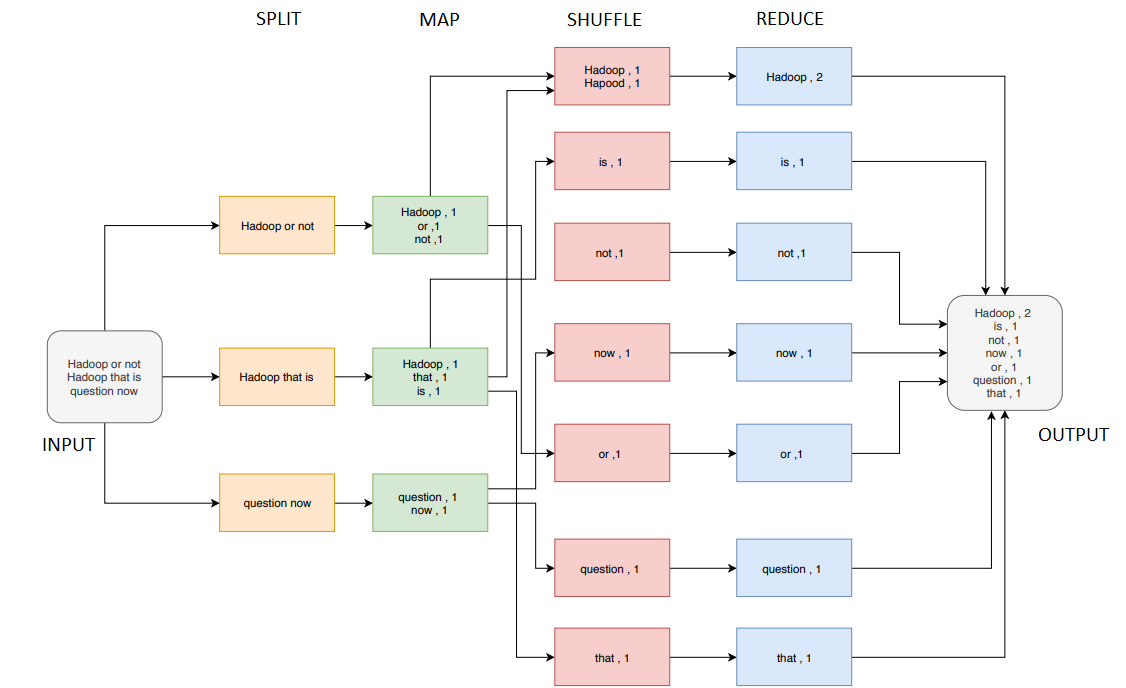
\includegraphics[width=0.8\linewidth]{Capture.PNG}\\
    \caption{Figure 1: MapReduce process} \\
\subsection{Summary at each stage}
 \begin{itemize}
 
     \item Split\\
     The process starts by distributing work among all available map nodes.
     \item Map\\
     Next, words are mapped and given a hard-coded value of "1" (this is done so as to count the number of times a word occurs)
     \item Shuffle\\
     During the shuffle phase, like words (keys) are separated and grouped together.
     \item Reducer\\
     The reducer sums the values within these individual groups of keys to produce a final output, that being, the number of times unique words appeared in text.
 \end{itemize}

\section{Code structure}

The following subsections give details about the algorithms implemented using the MapReduce framework. The framework chosen is Mrs.Mapreduce and thus requires to be coded in python. The code is centralized around the map and reduce operations that are provided by the framework, as is the focus the lab.  
\subsection{Word count}
The word count algorithm returns the frequency of each unique word within a piece of text while ignoring certain Stop words (this refers to commonly used words within a language e.g. for, as, the, etc).\\ Words were considered case-insensitive, this was done by converting all words to lower case before counting the number of times they appear. The code essentially maps each word to a value (which is always 1) and then shuffles and groups similar words in each process. Finally, the value associated with words with the same key are summed in order to obtain the total number of times that each word is seen in the text. The list of key value pairs are written to a text file for further processing.

\newline 

\subsection{Top-K query}
This piece of code returns the K most frequent words in a piece of text (K=10,20) while ignoring stop words. The top query requires the output of the word count algorithm. The text file produced by the previous algorithm is read and then sorted in descending order by value. The output is then the top K words and their frequencies that have been queried.  

\subsection{Inverted index}
The final algorithm concerns an inverted index. In computer science, inverted index can be understood as a database index that stores a map to content, such as words or numbers. The benefit of using inverted index is that it allows for fast full-text searches. \\
The implementation consists of listing each word with the line numbers that the word occurs. The inverted text algorithm makes use of a list to store page numbers, the constant value "50" is used to skip the first 50 lines of a file as it may include headings, dates, etc.\\
\newline
This algorithm consists of two processes. Firstly, instead of mapping each word to a value of 1, it is mapped to the line in which it occurs. This is done using the map and reduce functions in Mrs.MapReduce. In the reduce phase, the line numbers are not summed, but merely listed next to each word. Similarly the stop words as in the word count algorithm are ignored as well as digits occurring in the text. The output is then written to a text file for further processing. 

The next part involves reading the output from the map-reduce operations and then just formatting and selecting which part of the inverted index should be shown. 

%%%%%%%%%%%%%%%%%%%%%%%%%%%%%%%%%%%%%%%%%%%%%%%%%%%%%%%%%%%%%%%%%
\section{Results and Analysis}\

It was found through testing that all the algorithms worked as intended. The word count algorithm was able to successfully determined the frequency of unique words taking into consideration case sensitivity and ignoring stop words.\\
The top query algorithm successfully produced the top 10 and top 20 most frequent words.\\
The inverted index algorithm was able to correctly map words in text to the line numbers they appeared on. The algorithm produces more than 50 lines where some words occur, which can be fixed.  \\

Contained within the Appendix are snippets of the program output.
\newline

\section{Conclusion}

MapReduce iss designed to solve a major modern day problem, processing very large data sets, MapReduce is able to help solve this issue while also hiding the details of parrallelizing workflow and code. It has the  responsibility of executing written map and reduce functions in a distributed environment .\\
Mrs-MapReduce is one of many available MapReduce frameworks however from experience, Mrs-MapReduce proved to be an easy to use framework as well as being simple to install and configure. The report discusses three algorithms that use the MapReduce framework, namely; word count, top-k query and a modified inverted index. The algorithms perform as required on large text, thus showing how MapReduce is useful for sorting huge sets of data.


\justify

\begin{thebibliography}{9}
\bibitem{c1} Pythonhosted.org. (2019). User Guide — Mrs MapReduce v0.9 documentation. [online] Available at: https://pythonhosted.org/mrs-mapreduce/user\_guide.html [Accessed 16 Apr. 2019].



\end{thebibliography}


%%%%%%%%%%%%%%%%%%%%%%%%%%%%%%%%%%%%%%%%%%%%%%%%%%%%%%%%%%%%%%
\appendix
\newpage
\section{Appendix}
\subsection{Pseudo-code Lab 3}
%%%%%%%%%%%%%%%%%%%%%%%%%%%%%%%%%%%%%%%%%%%%%%%%%%%%%%%%%%%%%%
\begin{algorithm}[H]
\SetAlgoLined

definition map(self,key,value):\\
stop = [insert words to be excluded]\\
value = value.split()\\
value = [word.strip(string.punctuation).lower()]\\
\vspace{5pt}
\For{length of stop}{
 \While {stpWord in value}{
    value.remove(stpWord)
 }
}

\For{word in value}{
    \If{not str.isdigit(word)}{
        yield(word,1)
    }
}
\vspace{5pt}
definition reduce(self,key,values):\\
vals = sum(values)\\
yield vals


\caption{ Simple word count excluding stop words}
\end{algorithm}

%%%%%%%%%%%%%%%%%%%%%%%%%%%%%%%%%%%%%%%%%%%%%%%%%%%%%%%%%%%%%%
\begin{algorithm}[H]
\SetAlgoLined
Makes use of Algorithm 1\\

\vspace{10pt}
definition sortList(text):\\
text.sort(key= lambda x: x[1], reverse=True)\\
return text\\
\vspace{10pt}

definition top\_Kquery(text, k):\\
return(text[:k])\\
\vspace{10pt}	

definition process():	\\
cur\_ = os.getcwd()\\
dir\_ = os.path.join(cur_, "outdir")\\
fname = os.path.join(dir\_,"source\_0\_split\_0\_.mtxt")\\
f = open(fname, "r")\\
text = f.readlines()\\
\vspace{5pt}
\For{i in text}{
text[text.index(i)] = tuple(i.split()) }
return text
\vspace{10pt}	

        
definition main()\\
sorted\_txt = sortList(process())\\
query = [10,20]\\
\vspace{5pt}
\For{ k in query}{
print("Top: "+ str(k) + " occuring words")

\For{ i in top}{\_Kquery(sorted\_txt,k)\\
print(i)
}}

\caption{ Top K-query}
\end{algorithm}
%%%%%%%%%%%%%%%%%%%%%%%%%%%%%%%%%%%%%%%%%%%%%%%%%%%%%%%%%%%%%%


%%%%%%%%%%%%%%%%%%%%%%%%%%%%%%%%%%%%%%%%%%%%%%%%%%%%%%%%%%%%%%
\begin{algorithm}[H]
\SetAlgoLined

definition map(self,key,value):\\
stop = [insert words to be excluded]\\
value = value.split()\\
value = [word.strip(string.punctuation).lower()]\\
\vspace{5pt}
\For{length of stop}{
 \While {stpWord in value}{
    value.remove(stpWord)
 }
}

\For{word in value}{
line = value[0]\\
\vspace{5pt}
\If {not str.isdigit(word)}{
yield (word,line)}
}
\vspace{5pt}
definition reduce(self,key,values):\\
vals = sum(values)\\
yield vals


\caption{Algorithm line count}
\end{algorithm}

%%%%%%%%%%%%%%%%%%%%%%%%%%%%%%%%%%%%%%%%%%%%%%%%%%%%%%%%%%%%%%
\begin{algorithm}[H]
\SetAlgoLined
Makes use of Algorithm 3\\
\vspace{10pt}
definition lis_distinct(text,k):\\
return set(text[:k])\\
\vspace{10pt}

definition process(k):	\\
cur\_ = os.getcwd()\\
dir\_ = os.path.join(cur_, "outdir")\\
fname = os.path.join(dir\_,"source\_0\_split\_0\_.mtxt")\\
f = open(fname, "r")\\
text = f.readlines()\\
\vspace{5pt}
\For{line,i in enumerate(text)}{
\If{line > 50 and not re.search(r'/ d',i[0]}{
text[text.index(i)] = tuple(i.split()) \\
print(i)
}
\If{line==50}{break}

 }
\vspace{10pt}	

        
definition main()\\
k = 50\\
print("First distinct: "+ str(k) + " words")\\
fil = process(k)\\

\caption{ Inverted Index}
\end{algorithm}

\subsection{Program Output}
    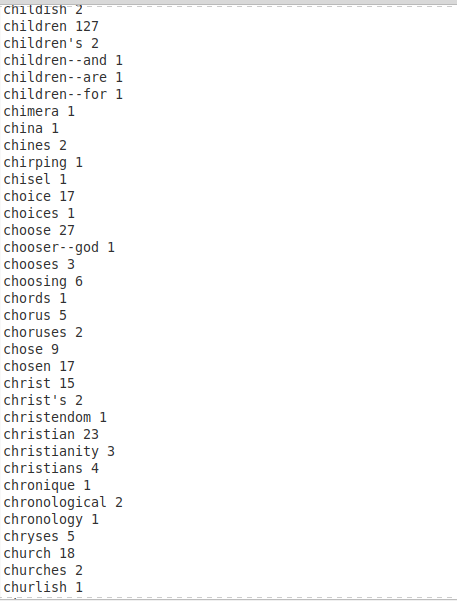
\includegraphics[width=0.55\linewidth]{wordcount.png}\\
    \caption{Figure 1: Word Count} \\
    
    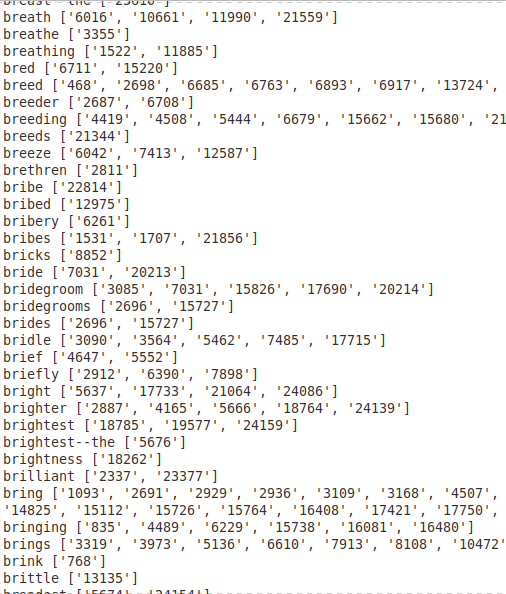
\includegraphics[width=0.55\linewidth]{inverted_index.png}\\
    \caption{Figure 2: Inverted Index} \\

\end{document}
